\chapter{Base Detection and Tracking}\label{chap:base_tracking}
One part of the work is focused on the state estimation of the moving platform. This is necessary in order to have a good prediction of the final state that the quadrotor must reach to land on the moving car. \\ 
With the method described in this section, every time we detect the platform, we can estimate its position, orientation and velocity in the world coordinate frame. Using this information as initial condition we can predict where the platform will be in $t$ seconds.\\
An EKF  \cite{kalmanfilter} is design in order to have the most reliable value of the state of the platform.\\

Kalman filtering consists in an algorithm that uses a series of noisy measurements observed over time and, using a model of  the dynamics of the system, produces estimates of unknown variables. This filter uses Bayesian inference and estimates a joint probability distribution over the variables for each time frame.\\

The algorithm works in a two-step process:
\begin{itemize}
\item in the prediction step, the KF produces estimates of the current state variables, along with their uncertainties, based on a model of the system:
\begin{align}
\boldsymbol{x}_k = f(\boldsymbol{x}_{k-1},\boldsymbol{u}_k) + \boldsymbol{w}_k
 \label{eq:ekf1} ;
\end{align} 
\item once the outcome of the next measurement is observed
\begin{align}
\boldsymbol{z}_k = h(\boldsymbol{x}_{k}) + \boldsymbol{v}_k
 \label{eq:ekf2} ,
\end{align}
these estimates are updated using a weighted average: the greater the weight the higher is the certainty of the measurement.
\end{itemize}
\newpage
In Eqs.~\eqref{eq:ekf1} and \eqref{eq:ekf2}
\begin{itemize}
\item $\boldsymbol{x}_k$ is the state to be estimated;
\item $\boldsymbol{z}_k$ the measure;
\item $\boldsymbol{u}_k$ the control input;
\item $f$ the state dynamics;
\item $h$ the measure model;
\item $\boldsymbol{w}_k$ and $\boldsymbol{v}_k$ the process and observation noises. These random variables are assumed to be multivariate Gaussian distribution with zero mean and covariances $\boldsymbol{Q}_k$ and $\boldsymbol{R}_k$ respectively.
\end{itemize}
In the EKF formulation the state transition $f$ and observation models $h$ do not need to be linear functions of the state but may instead be differentiable functions.\\

The algorithm is recursive and can run in real time, using only the current input measurements and the previously calculated state with its uncertainty matrix.
The KF does not require any assumption that the errors are Gaussian. However, the filter yields to the exact conditional probability estimate in the special case that all errors can be modeled as Gaussian distributions.\\

In the following we summarize the mathematical stages we have to perform in order to calculate the final estimate, in the case in which we have discrete time prediction and update models.\\
%Initialization
%\begin{align}
%\begin{split}
%\boldsymbol{x}_{0|0} = x_0\\
%\boldsymbol{P}_{0|0} = P_0
%\end{split}
%\end{align}
%For the prediction step of the EKF we have to solve:
%\begin{align}
%\begin{split}
%\boldsymbol{\dot{\hat{x}}}(t) &= f(\boldsymbol{\hat{x}}(t),\boldsymbol{u}(t)) \\
%\boldsymbol{\dot{P}}(t) &= \boldsymbol{F}(t) \boldsymbol{P}(t) + \boldsymbol{P}(t)\boldsymbol{F}(t)^{\top } + \boldsymbol{Q}(t)
%\end{split}
%\end{align}
%for $t \in (t_{k-1}, t_k)$ where
%\begin{align}
%\begin{split}
%\boldsymbol{\hat{x}}(t_{k-1}) &= \hat{x}_{k-1|k-1} \\
%\boldsymbol{P}(t_{k-1}) &= P_{k-1|k-1}
%\\
%{\boldsymbol{F}}(t)&=\left.{\frac  {\partial f}{\partial {\boldsymbol{x}}}}\right\vert _{{{\hat  {{\boldsymbol{x}}}}(t),{\boldsymbol{u}}(t)}}  \\
%\boldsymbol{\hat{x}}_{k|k-1} &= \boldsymbol{\hat{x}}(t_{k}) \\
%\boldsymbol{P}_{k|k-1} &= \boldsymbol{P}(t_{k})
%\end{split}
%\end{align}

\textbf{Initialization}:
\begin{subequations}
\begin{align}
\boldsymbol{\hat{x}}_{0|0} = x_0 ,  \\[10pt]
\boldsymbol{P}_{0|0} = P_0 .
\end{align}
\end{subequations}

\textbf{Prediction step}:
\begin{subequations}
\begin{align}
\boldsymbol{\hat{x}}_{k|k-1} &= f(\boldsymbol{\hat{x}}_{k-1|k-1},\boldsymbol{u}_k), \\[10pt]
\boldsymbol{P}_{k|k-1} &= \boldsymbol{F}_{k-1} \boldsymbol{P}_{k-1|k-1}\boldsymbol{F}_{k-1}^{\top } + \boldsymbol{Q}_{k},
\end{align}
\end{subequations}
where the state transition matrix is defined to be the following Jacobians:
\begin{align}
\boldsymbol{F}_{k-1}&= \left.{\frac{\partial f}{\partial {\boldsymbol{x}}}} \right \vert_{\hat{\boldsymbol{x}}_{k-1|k-1},\boldsymbol{u}_{k}}.
\end{align}

\textbf{Update step}: 
\begin{subequations}
\begin{align}
\boldsymbol{K}_{k} &= \boldsymbol{P}_{k|k-1} \boldsymbol{H}_{k}^{\top }(\boldsymbol{H}_{k} \boldsymbol{P}_{k|k-1} \boldsymbol{H}_{k}^{\top }+ \boldsymbol{R}_{k})^{-1}, \\[10pt]
\hat{\boldsymbol{x}}_{k|k} &= \hat{\boldsymbol{x}}_{k|k-1} + \boldsymbol{K}_{k} (\boldsymbol{z}_{k}-h(\hat{\boldsymbol{x}}_{k|k-1})) ,\\[10pt]
\boldsymbol{P}_{k|k} &=(\boldsymbol{I}-\boldsymbol{K}_{k}\boldsymbol{H}_{k})\boldsymbol{P}_{k|k-1} ,
\end{align}
\end{subequations}
where the observation matrix is defined to be the following Jacobian:
\begin{align}
\boldsymbol{H}_{k} = \left.{\frac{\partial h}{\partial {\boldsymbol{x}}}} \right \vert_{\hat{\boldsymbol{x}}_{k|k-1}}.
\end{align}

\section{Prediction update: non-holonomic model}
The platform is considered as a car and simulated with the non-holonomic model Fig.~\ref{fig:nonholonomicmodel} and Eq.~\ref{eq:equation_nonholonomic_continuos}.\\
In this model, the state is defined as $\boldsymbol{x} = (x, y, z,\theta , v_{tan}, \phi)$: it corresponds to the 3 position in a space $(x,y,z)$,  the yaw angle of the platform $(\theta)$ with respect to the world frame, the forward velocity ($v_{tan}$), and the angle of the front wheels ($\phi$). The system depends on a parameter $L$ that corresponds to the distance between the front and the back wheels.\\
In this model the control input are the change in velocity $u_1 = \dot{v}_{tan}$ and in the angle of curvature $u_2 = \dot{\phi}$. \\
\begin{figure}[!ht]
    \centering
    \includegraphics[width=0.5\textwidth]{img/non_holonomic_model.png}
    \caption{Non-holonomic model}
    \label{fig:nonholonomicmodel}
\end{figure}

The equation of motion in continuous time are:
\begin{align}
\boldsymbol{\dot{x}}  = 
\begin{bmatrix}
\dot{x}  \\[10pt]
\dot{y}  \\[10pt]
\dot{z} \\[10pt]
\dot{\theta} \\[10pt]
\dot{v_{tan}}  \\[10pt]
\dot{\phi}
\end{bmatrix}
= 
\begin{bmatrix}
v_{tan} cos(\theta) \\[10pt]
v_{tan} sin(\theta) \\[10pt]
 0 \\[10pt]
\frac{v_{tan}}{L}tan(\phi)\\[10pt]
u_1 \\[10pt]
 u_2 
\end{bmatrix}
=  f(\boldsymbol{x},\boldsymbol{u})
\label{eq:equation_nonholonomic_continuos}
\end{align}
It is possible to discretize these dynamics with first order finite difference:
\begin{align}
\boldsymbol{\dot{x}} \approx \frac{\boldsymbol{x}(t_k)- \boldsymbol{x}(t_{k-1}) }{ t_k - t_{k-1}} = \frac{\boldsymbol{x}_k - \boldsymbol{x}_{k-1} }{dt} \approx f(\boldsymbol{x}_{k-1},\boldsymbol{u}_k).
\end{align}
This leads to:
\begin{align}
\boldsymbol{x_k} = 
\begin{bmatrix}
x_k  \\[10pt]
y_k  \\[10pt]
z_k \\[10pt]
\theta_k \\[10pt]
v_{tan,k}  \\[10pt]
\phi_k
\end{bmatrix}
= 
\begin{bmatrix}
 x_{k-1} + dt \big(v_{tan,k-1} cos(\theta_{k-1})\big) \\[10pt]
 y_{k-1} + dt \big(v_{tan,k-1} sin(\theta_{k-1})\big) \\[10pt]
 z_{k-1} \\[10pt]
 \theta_{k-1} + dt\Big(\frac{v_{k-1}}{L}tan(\phi_{k-1}) \Big)\\[10pt]
v_{tan,k-1} + dt \big(u_{1,k}\big) \\[10pt]
\phi_{k-1} + dt \big(u_{2,k}\big) 
\end{bmatrix}
\label{eq:equation_nonholonomic_discrete}
\end{align}

In order to solve the former system a numerical solution is necessary. For this purpose we use a Runge-Kutta scheme  \cite{wiki_runge_kutta}.\\
In numerical analysis, the Runge-Kutta methods are a family of implicit and explicit iterative methods used in temporal discretization for the approximate solutions of ordinary differential equations.\\
The most widely known member of the Runge-Kutta family is generally referred to as RK4.\\
Let an initial value problem be specified as follows:
\begin{align}
\begin{cases}
\boldsymbol{\dot {y}} =f(\boldsymbol{y},t) \\[10pt]
\boldsymbol{y}(t_{0}) =\boldsymbol{y}_{0}
\end{cases},
\end{align}
where $\boldsymbol{y}$ is an unknown function of time $t$, which we want to approximate, and the function $f$ and the data $t_{0}$, $\boldsymbol{y}_{0}$ are given.\\
Now we want to discretize the dynamics in the interval $t \in [0,T]$. We choose a step size $h > 0$ such that the interval is divided in $N$ sub-intervals. For each of these we define:
\begin{align}
\begin{cases}
\boldsymbol{y}_{k+1}&=\boldsymbol{y}_{k}+{\tfrac {h}{6}}\left(\alpha_{1}+2\alpha_{2}+2\alpha_{3}+\alpha_{4}\right)\\[10pt]
t_{k+1}&=t_{k}+h
\end{cases} \ \ \ \ \ \  \forall k \in [0,N] ,
\end{align}
where:
\begin{align}
\begin{cases}
\alpha_{1}&=f\Big(\boldsymbol{y}_{k},t_{k}\Big)\\[10pt]
\alpha_{2}&=f\Big(\boldsymbol{y}_{k}+{\frac {h}{2}}\alpha_{1},t_{k}+{\frac {h}{2}}\Big)\\[10pt]
\alpha_{3}&=f\Big(\boldsymbol{y}_{k}+{\frac {h}{2}}\alpha_{2},t_{k}+{\frac {h}{2}}\Big)\\[10pt]
\alpha_{4}&=f\Big(\boldsymbol{y}_{k}+h\alpha_{3},t_{k}+h\Big)
\end{cases}
\end{align}
With this algorithm we calculate  $\boldsymbol{y}_{k+1}$: the RK4 approximation of $\boldsymbol{y}(t_{k+1})$. As explained this quantity is determined by the sum of current value $\boldsymbol{y}_{k}$ and the weighted average of four increments.

\subsection{Straight and circular path} \label{subsec:circularlinearmodel}
If we assume that the input $u_{1,k}$ and $u_{2,k}$ are equal to zero $\forall k$ we can have three types of movement:
\begin{itemize}
\item the platform can be static ($v_{tan,0} = 0$);
\item it can move in a straight line ($v_{tan,0} \neq 0$ and $\phi_0 = 0$);
\item it can move in a circle ($v_{tan,0} \neq 0$ and $\phi_0 \neq 0$).
\end{itemize}
A combination of these type of movements, even if they are really simple, leads to a large set of possible trajectories.\\
Furthermore, when we use this model in the prediction step of the EKF, we consider that it is corrupted by Gaussian noise. This way a modification in the control inputs $u_{1,k}$ and $u_{2,k}$ can be part of the model as far as it is slow and smooth.\\

\subsection{Infinity shape path}
As described in Chapter \ref{chap:thechallenge}, the moving platform moves in an infinity-shape path described in Fig.~\ref{fig:arenachallenge}. \\
We need to describe in a mathematical way this shape in order to use this information when we are estimating the state of the platform and to understand the right moment to perform the landing maneuver.\\
From the specification of the challenge:
\begin{itemize}
\item the car is moving with constant velocity $v_{tan}$ along the path;
\item the radius of the circumferences that forms the trajectory is $\rho_{8} =$ \SI{20}{\meter};
\item the path makes a cross in the middle that creates 4 angles of $\frac{\pi}{2}$. 
\end{itemize}
It easy to see that the shape can be seen as a combination of a cross and two circles.
If we consider the world coordinate system, this path can be located in any position with any orientation in the $x,y$ plane. To describe mathematically the trajectory, we consider that the center of the cross is in the origin of the world coordinate frame. Then, if we want to model the real world path, we apply a rigid transformation in the $x,y$ plane.\\

The cross is simply defined as the union between the two line:
\begin{subequations}
\begin{align}
y &= x \\[5pt]
y &= -x \ \ \  ,
\end{align}
\end{subequations}
while the two circles can be modeled as:
\begin{subequations}
\begin{align}
y^2 + (x - x_0)^2 &= \rho_{8}^2 \\[10pt]
y^2 + (x + x_0)^2 &= \rho_{8}^2 
\end{align}
\end{subequations}
It easy to see from Fig. \ref{fig:constuctinfinity} that if we want the intersections between the cross and the two circumferences to be exactly in 4 points we have to choose:
\begin{align}
x_0 = \frac{\sqrt{2}}{2}\rho_{8}
\end{align}
This corresponds to the 4 intersections coordinate:
$$
\Big(\frac{\rho_{8}\sqrt{2}}{2},\frac{\rho_{8}\sqrt{2}}{2}\Big); \ 
\Big(\frac{\rho_{8}\sqrt{2}}{2},-\frac{\rho_{8}\sqrt{2}}{2}\Big); \
\Big(-\frac{\rho_{8}\sqrt{2}}{2},-\frac{\rho_{8}\sqrt{2}}{2}\Big); \
\Big(-\frac{\rho_{8}\sqrt{2}}{2},\frac{\rho_{8}\sqrt{2}}{2}\Big).
$$

\begin{figure}[!htbp]
 \centering
   \begin{subfigure}[b]{0.45\textwidth}
     \includegraphics[width=\textwidth]{img/constructionshape1_.png}
        \label{fig:constuctinfinity1}
   \end{subfigure}
   \hfill
   \begin{subfigure}[b]{0.45\textwidth}
     \includegraphics[width=\textwidth]{img/constructionshape2_.png}
       \label{fig:constuctinfinity2}
   \end{subfigure}
   \caption{How to construct the infinity-shape path}
   \label{fig:constuctinfinity}
 \end{figure} 
  
The easiest way to describe this path is to define how the angle $\theta$ is changing along the trajectory. If we travel over the two circumferences the intersections correspond to angles $\theta = \pm \frac{3\pi}{4}$. \\
Now it is obvious to see that the path is symmetric and it can be divided in 4 parts and, describing how the angle is changing in one of this section, the whole trajectory is defined.\\
We can observe that if $x$ is the space traveled along the infinity path:
\begin{align}
\theta(x) =
\begin{cases}
    -\frac{x}{\rho_{8}}  &x\in \Big[0,\frac{3\pi}{4}\rho_{8}\Big] \quad \quad \ \ \  \\[10pt]
    -\frac{3\pi}{4} &x\in \Big[\frac{3\pi}{4}\rho_{8} ,\frac{3\pi}{4}\rho_{8} + \rho_{8}\Big]
\end{cases}
\end{align}
This function defines a quarter of the trajectory in function of the radius $\rho_{8}$ of the path. Figure~\ref{fig:quarter_xy} shows the shape of this quarter of trajectory.\\
It is now possible to use it to generate the entire trajectory $\big(x(t), y(t)\big)$ described in Fig.~\ref{fig:entire_xy2}.\\
We know that the length of the path is 
\begin{align}
l = 4\Big(\frac{3\pi}{4}\rho_{8} + \rho_{8}\Big),
\end{align}
and given the constant velocity $v_{tan}$ we can calculate the time to complete the trajectory as:
\begin{align}
T = \frac{l}{v_{tan}}.
\end{align}
Also, it is simple to define $\theta(t)$ just stretching or shrinking $\theta(x)$. So we can now define:
\begin{align}
\begin{cases}
\dot{x} = v_{tan} cos\big(\theta(t)\big) \\[10pt]
\dot{y} = v_{tan} sin\big(\theta(t)\big)
\end{cases}
\end{align}
Finally, we also need the discretized version obtained just using forward Euler approximation:
\begin{align}
\begin{cases}
x_k = x_{k-1} + dt \Big(v_{tan,k-1} cos\big(\theta_{k-1}\big)\Big) \\[10pt]
y_k = y_{k-1} + dt \Big(v_{tan,k-1} sin\big(\theta_{k-1}\big)\Big)
\end{cases}
\end{align}
\begin{figure}[!htbp]
 \centering
   \begin{subfigure}[b]{0.42\textwidth}
     \includegraphics[width=\textwidth]{img/angle_x.eps}
        \caption{Angle in function of the space}
        \label{fig:quarter_theta}
   \end{subfigure}
   \hfill
   \begin{subfigure}[b]{0.45\textwidth}
     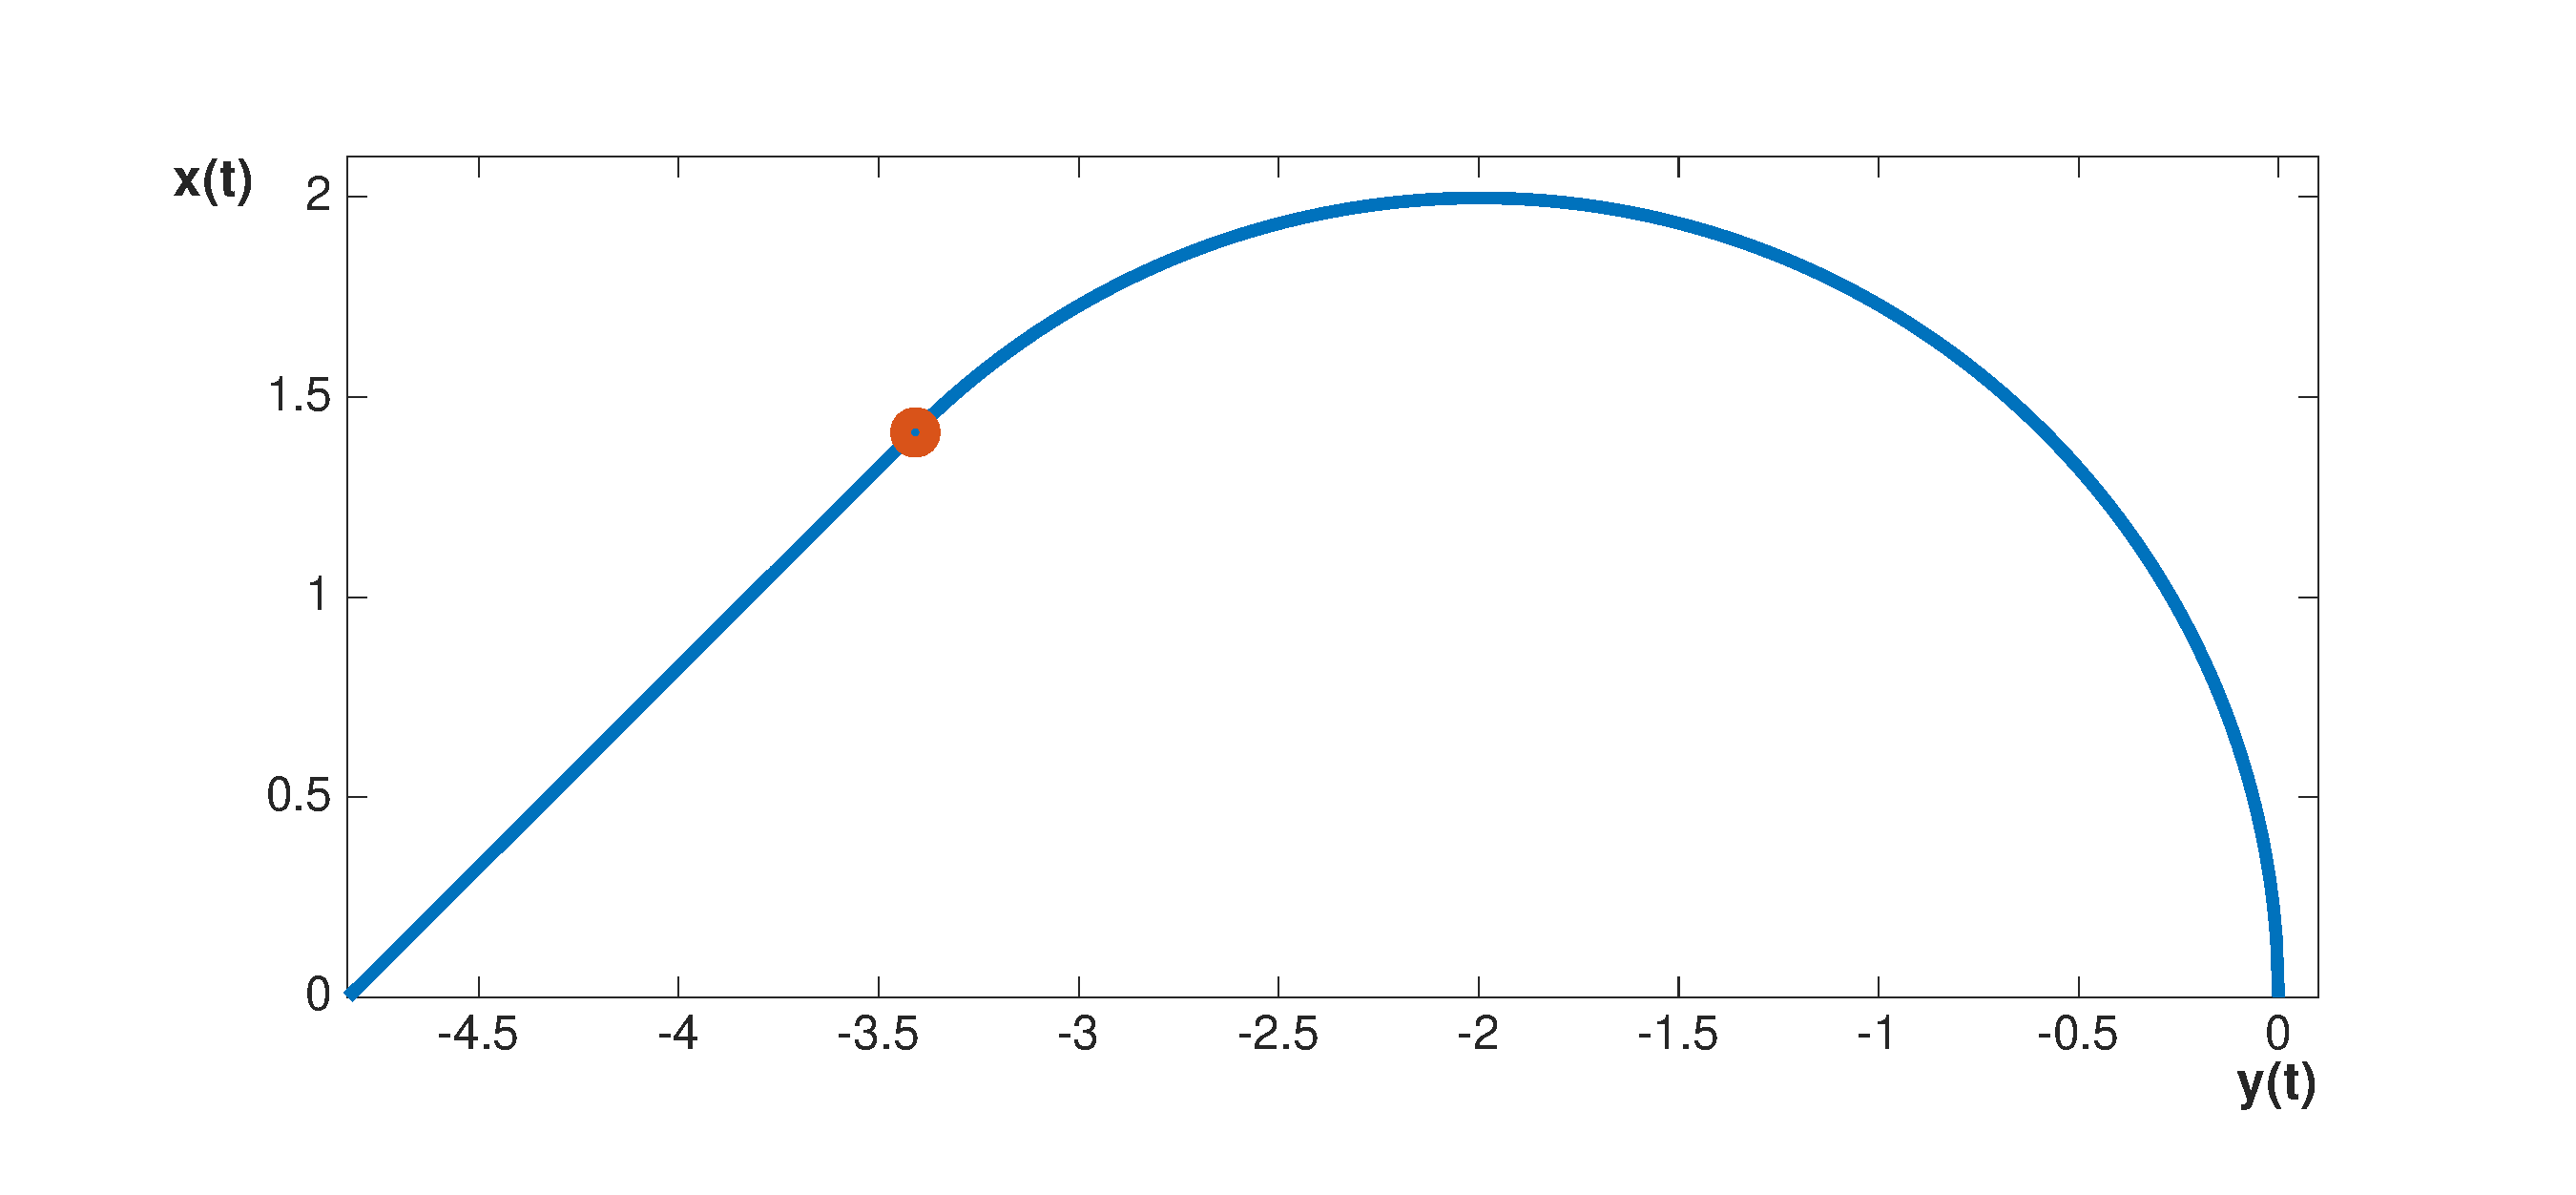
\includegraphics[width=\textwidth]{img/path_x_quarter.eps}
        \caption{One quarter of the path}
       \label{fig:quarter_xy}
   \end{subfigure}
   
   \begin{subfigure}[b]{0.45\textwidth}
     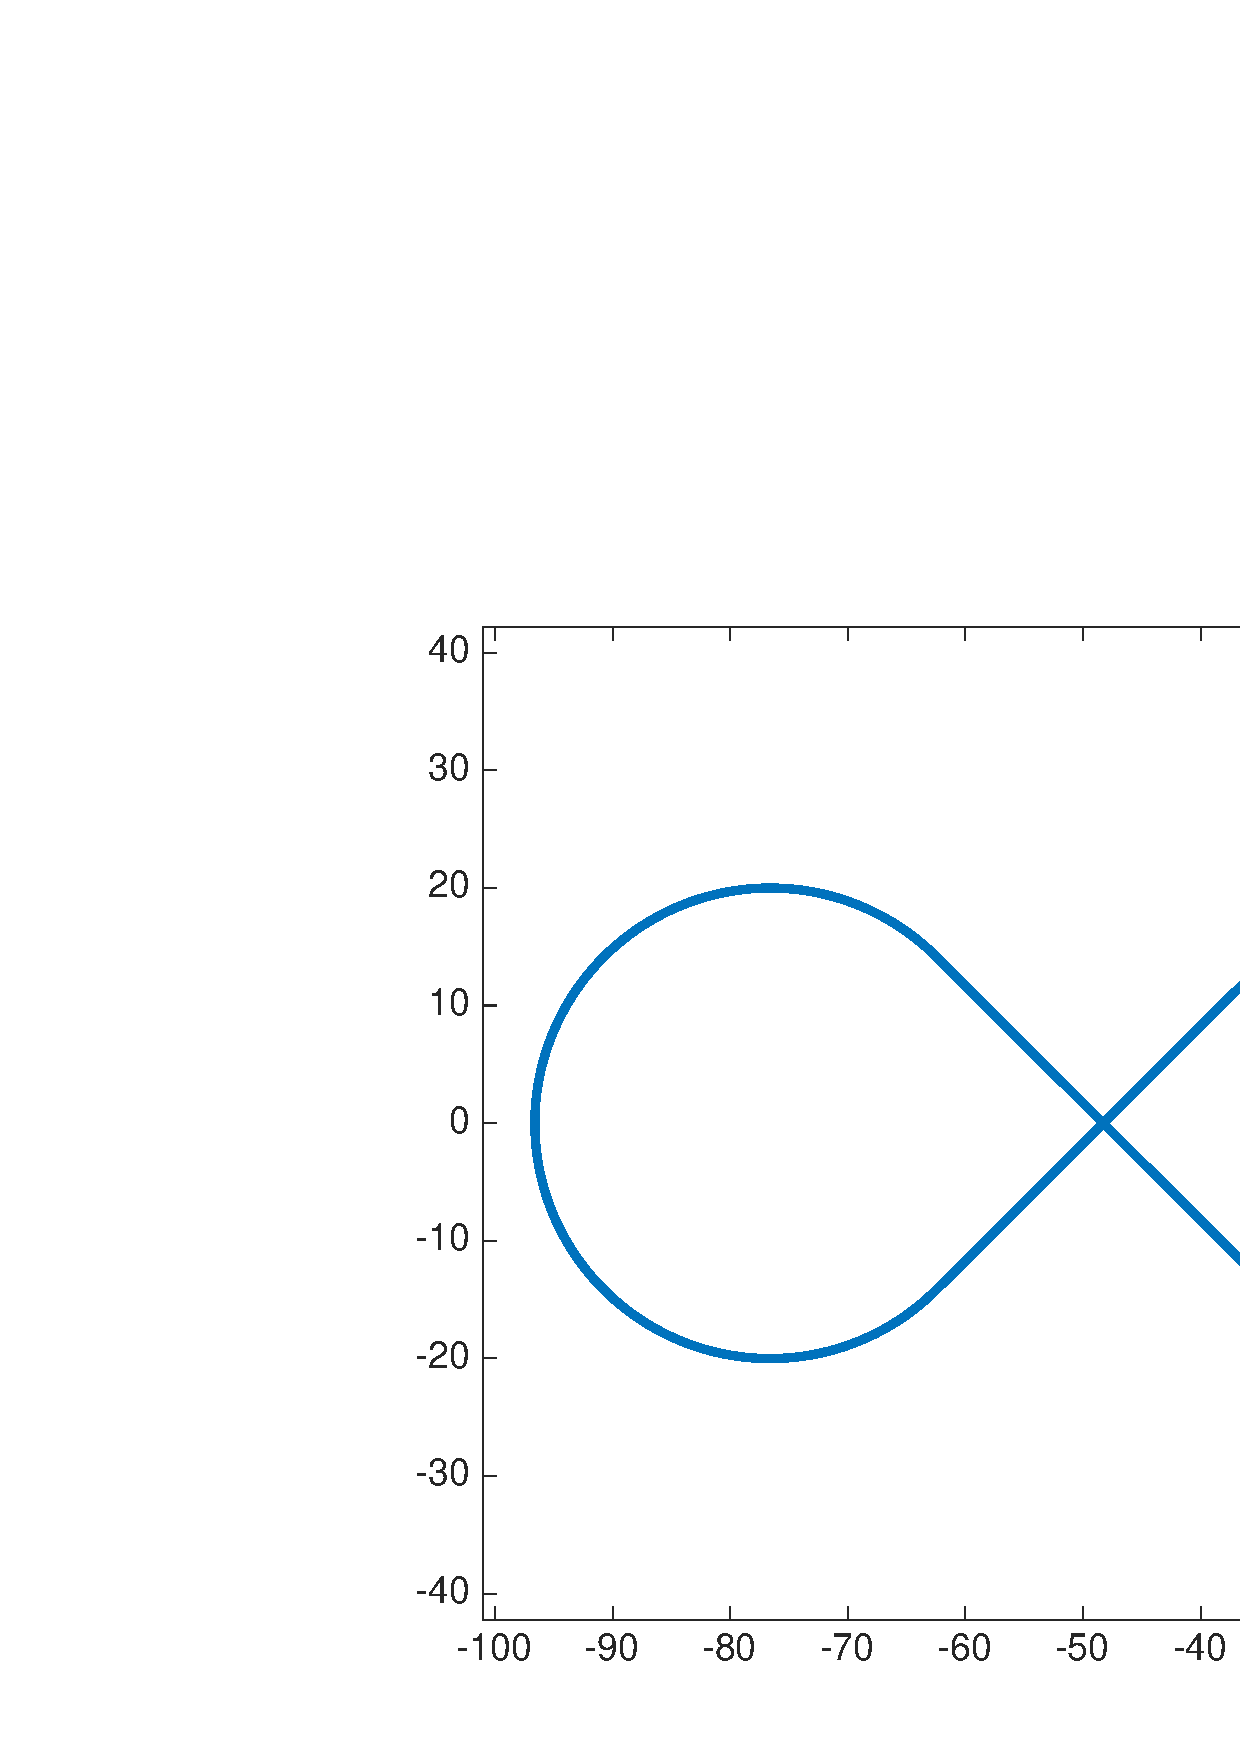
\includegraphics[width=\textwidth]{img/infinityshapepath.png}
        \caption{The whole the path}
       \label{fig:entire_xy2}
   \end{subfigure}
    \caption{The parametrization of the path}
  \label{fig:path}
  \end{figure}
  
From these calculations we can conclude that the final trajectory of the platform is only a composition of a linear and a circular movement (for a given amount of time). So the model described in Sec. \ref{subsec:circularlinearmodel} can be used also to express this trajectory.

\section{Measurement update}
From Eq.~\eqref{eq:equation_nonholonomic_discrete} we have the variables that describe the state of the moving car. We have to be able to measure some of these components in order to perform the second step of our EKF. \\
We use a down looking camera to identify the moving platform and to estimate its position and orientation. At this point, knowing the position of the camera in the real world we can measure:
\begin{align}
\boldsymbol{z}_k = h(\boldsymbol{x}_k) =
\begin{bmatrix}
1 & 0 & 0 & 0 & 0 & 0 \\[10pt]
0 & 1 & 0 & 0 & 0 & 0  \\[10pt]
0 & 0 & 1 & 0 & 0 & 0 \\[10pt]
0 & 0 & 0 & 1 & 0 & 0
\end{bmatrix} 
\begin{bmatrix}
x_k \\[5pt]
y_k  \\[5pt]
z_k \\[5pt]
\theta_k \\[5pt]
v_{tan,k} \\[5pt]
\phi_k
\end{bmatrix} = \begin{bmatrix}
x_k  \\[10pt]
y_k  \\[10pt]
z_k \\[10pt]
\theta_k
\end{bmatrix}
\label{eq:realmeasure}
\end{align}
It corresponds to the 3 position in a space $(x,y,z)$ and the yaw angle of the platform $\theta$ with respect to the world frame.

In Chap. \ref{chap:area_exploration} we will see that in order to complete the task, the quadrotor goes through various stages. In these different phases the relative distance between camera and moving platform changes a lot, so we have to use different methods to measure $\boldsymbol{z}$:
\begin{itemize}
\item to be able to find the platform in the minimum amount of time, at the beginning, we need to inspect the area from a very high altitude. From this height we can see only a few features of the moving car and then the pose estimation is really noisy. Furthermore, we do not have any assumption on the initial condition of the platform, but we just know the magnitude of constant forward velocity $|v_{tan}|$. Therefore, we do not know in advance if at a certain time $t$ the car is moving on a straight line or in a curve. This renders necessary to observe the moving platform for several seconds in order to determine on which part of the track it is.
\item After knowing the type of movement and a rough pose estimation of the moving car, we can use these information to improve our state estimation: getting close to the platform without loosing the tracking, a more precise measure is available (base on tag detection), and filtering the measurements with the correct theoretical model of the movement.
\end{itemize}

\subsection{Platform pose estimation at high altitudes}
To find the car, we assume that the platform is the only white square moving on the arena.\\
Based on this assumption, we analyze the images from the camera to find a moving white square and calculate its optical flow to predict its future position.\\
To find the base we perform the following steps:
\begin{itemize}
\item thresholding the image in order to find the white blobs;
\item finding all the close shapes in the image;
\item selecting only the shapes having:
\begin{itemize}
\item 4 edges;
\item convex contour;
\item angles between edges close to $\frac{\pi}{2}$.
\end{itemize}
\end{itemize}
At this point, we have the position of the four corners of the squares in the image.\\

Now we calculate the optical flow of these points through the sequence of images and we track only the points that are moving with a velocity comparable to the one known $v_{tan}$.\\
The optical flow methods \cite{beauchemin1995computation} calculate the motion of each pixel between two subsequent images.
For a 2D case, a pixel at location $(x,y,t)$ with intensity $I(x,y,t)$ moves by $\Delta x$,$\Delta y$ and $\Delta t$ between the two image frames. To solve this problem, the core assumption is the brightness constancy constraint:
\begin{align}
I(x,y,t) = I(x+\Delta x, y + \Delta y, t + \Delta t)
\end{align}
Assuming the movement to be small, the image constraint at $I(x,y,t)$ can be approximated with its first order Taylor Series:
\begin{align}
I(x+\Delta x,y+\Delta y,t+\Delta t) \simeq I(x,y,t) + \frac{\partial I}{\partial x}\Delta x+\frac{\partial I}{\partial y}\Delta y+\frac{\partial I}{\partial t}\Delta t.
\end{align}
It follows that:
\begin{align}
 \frac{\partial I}{\partial x}\frac{\Delta x}{\Delta t}+\frac{\partial I}{\partial y}\frac{\Delta y}{\Delta t}+\frac{\partial I}{\partial t}\frac{\Delta t}{\Delta t} = 0,
\end{align}
which results in:
\begin{align}
 I_{x}V_x+I_{y}V_y+I_{t}= 0,
\end{align}
where $V_x,V_y$ are the $x$ and $y$ components of the velocity, or optical flow, of $I(x,y,t)$, and $I_{x}$, $I_{y}$, $I_{t}$ are the derivatives of the image at $(x,y,t)$ in the corresponding directions.\\
Thus in a compact form:
\begin{align}
 \nabla I^T\cdot\vec{V} = -I_t
\end{align}
This is a single equation in two unknowns and cannot be solved as such. This is known as the aperture problem of the optical flow algorithms. To find the optical flow another set of equations is needed, given by some additional constraint. All optical flow methods introduce additional conditions for estimating the actual flow.\\
In our implementation we use the Lucas-Kanade method \cite{lucas1981iterative}. This method assumes that the displacement of the image contents between two nearby frames is small and approximately constant within a neighborhood of the point $p$ under consideration. Thus the optical flow equation can be assumed to hold for all pixels within a window centered at $p$. Namely, the local image flow vector $(V_{x},V_{y})$ must satisfy:
\begin{align}
\begin{cases}
I_{x}(q_{1})V_{x}+I_{y}(q_{1})V_{y}=-I_{t}(q_{1})  \\[10pt]
I_{x}(q_{2})V_{x}+I_{y}(q_{2})V_{y}=-I_{t}(q_{2})  \\[10pt]
\ \ \ \ \ \vdots \\[10pt]
I_{x}(q_{n})V_{x}+I_{y}(q_{n})V_{y}=-I_{t}(q_{n}) 
\end{cases}
\end{align}

Where $q_{1},q_{2},\dots ,q_{n}$ are the pixels inside the window, and $I_{x}(q_{i}),I_{y}(q_{i}),I_{t}(q_{i})$ are the partial derivatives of the image $I$ with respect to position $x, y$ and time $t$, evaluated at the point $q_{i}$ and at the current time.\\
These equations can be written in matrix form $Av=b$, where
\begin{align}
\boldsymbol{A}={\begin{bmatrix}I_{x}(q_{1})&I_{y}(q_{1})\\[10pt]I_{x}(q_{2})&I_{y}(q_{2})\\[10pt]\vdots &\vdots \\[10pt]I_{x}(q_{n})&I_{y}(q_{n})\end{bmatrix}} \quad \quad \boldsymbol{v}={\begin{bmatrix}V_{x}\\[10pt]V_{y}\end{bmatrix}} \quad \quad \boldsymbol{b}={\begin{bmatrix}-I_{t}(q_{1})\\[10pt]-I_{t}(q_{2})\\[10pt]\vdots \\[10pt]-I_{t}(q_{n})\end{bmatrix}}
\end{align}

This system has more equations than unknowns and thus it is usually over-determined. The Lucas-Kanade method obtains solution by using the least squares method:
\begin{subequations}
\begin{align}
\boldsymbol{A}^{T}\boldsymbol{Av}=\boldsymbol{A}^{T}\boldsymbol{b}\\[10pt]
{\boldsymbol{v}}=(\boldsymbol{A}^{T}\boldsymbol{A})^{{-1}}\boldsymbol{A}^{T}\boldsymbol{b}
\end{align}
\end{subequations}
\begin{align}
{\begin{bmatrix}
V_{x}\\[10pt]
V_{y}\end{bmatrix}}
=
{\begin{bmatrix}
\sum _{i}I_{x}(q_{i})^{2}&\sum _{i}I_{x}(q_{i})I_{y}(q_{i})\\[10pt]
\sum _{i}I_{y}(q_{i})I_{x}(q_{i})&\sum _{i}I_{y}(q_{i})^{2}
\end{bmatrix}}^{{-1}}
{\begin{bmatrix}
-\sum _{i}I_{x}(q_{i})I_{t}(q_{i})\\[10pt]
-\sum _{i}I_{y}(q_{i})I_{t}(q_{i})
\end{bmatrix}}
\end{align}

With this method we can track the interesting points, namely the platform corners, from frame to frame and calculate the direction and velocity of their movement. We need now a method to convert this position in the image into the correspondent pose in the real world.

\subsubsection{From images to real world}
After tracking the platform in the images, we have to find its position in the 3D real world. This position is calculated using the pinhole model of the camera \cite{weng1992camera}:
\begin{subequations}
\begin{align}
\omega \boldsymbol{m} \ \ & = \boldsymbol{A} [\boldsymbol{R}|\boldsymbol{t}]\boldsymbol{M} \\[10pt]
{\omega \begin{bmatrix}
u \\[10pt]
v  \\[10pt]
1
\end{bmatrix}} & =
{\begin{bmatrix}\
f_x & 0 & c_x \\[10pt]
0 & f_y &c_y \\[10pt]
0 & 0 & 1
\end{bmatrix}}
{\begin{bmatrix}\
r_{11} & r_{12} & r_{13} & t_{x} \\[10pt]
r_{21} & r_{22} & r_{23} & t_{y} \\[10pt]
r_{31} & r_{32} & r_{33} & t_{z}
\end{bmatrix}}
{\begin{bmatrix}
X \\[5pt]
Y \\[5pt]
Z \\[5pt]
1
\end{bmatrix}}
 \label{eq:pinholemodel}
\end{align}
\end{subequations}
Where:
\begin{itemize}
 \item $\boldsymbol{m}$: is the homogeneous coordinate of the point in the image expressed in pixel $(u,v,1)$;
  \item $\boldsymbol{M}$: is the homogeneous coordinate of the correspondent 3D point in the world coordinate frame $(X,Y,Z,1)$;
 \item $\boldsymbol{A}$: is the camera matrix, or the matrix of intrinsic parameters. It is composed by the focal lengths $f_x,f_y$  and the principal point $c_x,c_y$;
 \item $[\boldsymbol{R}|\boldsymbol{t}]$: is the joint rotation-translation matrix, or matrix of extrinsic parameters. It expresses the camera motion around the static scene. This matrix denotes the pose of the camera in the world frame. In particular, we have to notice that the position $\boldsymbol{C}$ of the camera expressed in world coordinates is $\boldsymbol{C}=-\boldsymbol{R}^{{-1}}\boldsymbol{t}=-\boldsymbol{R}^{T}t$.
\end{itemize}

We can calculate the depth of the platform using the known dimension of the base: given the length $l_w$ of the square in the real world and the average dimension of the edges in the image $l_i$, we can calculate the depth with respect to the camera frame 
\begin{align}
z = \frac{l_w f}{l_i}
\end{align}
To calculate the dimension $l_i$ we need at least 3 corner of the base and we calculate all the pairwise distances between the corners (c.f. Fig. \ref{fig:platform_profile}):
\begin{itemize}
\item if we have 4 corners there are 6 different distances: 4 of which equal to $l_i$ and 2 $\sqrt{2}l_i$ (Fig. \ref{fig:4_corners} );
\item if we have 3 corners there are 3 different distances: 2 of which equal to $l_i$ and 1 $\sqrt{2}l_i$  (Fig. \ref{fig:3_corners} ).
\end{itemize}

\begin{figure}[!htbp]
  \centering
   \begin{subfigure}[b]{0.3\textwidth}
        \includegraphics[width=\textwidth]{img/platform_4_edges.pdf} 
        \caption{4 corners of the base are in the f.o.v} 
                \label{fig:4_corners}
   \end{subfigure}\hspace{5em}
   \begin{subfigure}[b]{0.3\textwidth}
        \includegraphics[width=\textwidth]{img/platform_3_edges.pdf}
        \caption{3 corners of the base are in the f.o.v}
        \label{fig:3_corners}
   \end{subfigure}
   
   \caption{Model of the square platform detected on the image. Red crosses corner detected. Blue lines edges with length $l_i$. Green lines edges with length $\sqrt{2}l_i$ }
  \label{fig:platform_profile}
\end{figure} 

Although this approximation is not accurate when we see the platform with a camera not perpendicular to the base, we use it to have a rough approximation of the height in this first phase. Since the distance between camera and platform is very high, this assumption can hold.\\

If this depth $z$ is nonzero, we can  solve the system of equation \eqref{eq:pinholemodel} to find an unique solution using the following equivalent equations:
\begin{subequations}
\begin{align}
&x = z\frac{u-c_x}{f_x}\\[10pt]
&y = z\frac{v-c_y}{f_y}\\[10pt]
&{\begin{bmatrix}
x \\[10pt]
y \\[10pt]
z
\end{bmatrix}} = 
\boldsymbol{R} {\begin{bmatrix}
X \\[10pt]
Y \\[10pt]
Z
\end{bmatrix}} + \boldsymbol{t}
\end{align}
\end{subequations}

As previously said, this method is not very accurate, because we are assuming that the platform surface and the image plane are parallel.
A better method to find the position of the platform, without the approximation of the depth $z$, is to resolve a Perspective-n-Point problem  \cite{quan1999linear} that estimates the pose of a camera given a set of $n$ 3D points in the world and their corresponding 2D projections in the image. This method finds the pose that minimize the reprojection error of the 3D points in the image plane.\\
The main issue is that, to solve this problem, without ambiguity, the minimum number of points is 4, and sometimes we can track only 3 corners of the base. Therefore when all the 4 points are available we solve the correspondent PnP problem to find a better estimation of the base position, otherwise we use the former method.\\

At this point, with this algorithm, we can track the points of interest from frame to frame, the calculate direction, the velocity and the correspondent 3D pose of the car.\\

\begin{figure}[!htbp]
  \centering
   \begin{subfigure}[b]{0.45\textwidth}
        \includegraphics[width=\textwidth]{img/img_330.png}
        \label{fig:one_1}
        \caption{}
   \end{subfigure}\hfill
   \begin{subfigure}[b]{0.45\textwidth}
        \includegraphics[width=\textwidth]{img/img_155.png}
        \label{fig:two_1}
        \caption{}
   \end{subfigure}
%    \begin{subfigure}[b]{0.45\textwidth}
%        \includegraphics[width=\textwidth]{img/img_330.png}
%        \label{fig:two_1}
%   \end{subfigure}
  \caption{Real world example. The center of the platform is calculated detecting the white square and its corners. In figure (a) all the 4 corners of the base are visible in the image, while in figure (b) only 3 are in the field of view. With the algorithm described in both cases we can calculate the position of the center.}
  \label{fig:optical_folw_sequence2}
\end{figure} 

\begin{figure}[!htbp]
  \centering
   \begin{subfigure}[b]{0.45\textwidth}
        \includegraphics[width=\textwidth]{img/18730previousImage.png}\label{fig:original}
        \caption{}
   \end{subfigure}  \hfill
   \begin{subfigure}[b]{0.45\textwidth}
        \includegraphics[width=\textwidth]{img/18730_thresholded.png}\label{fig:threshold}
        \caption{}
   \end{subfigure}
   
    \begin{subfigure}[b]{0.45\textwidth}
        \includegraphics[width=\textwidth]{img/18741_optical_flow.png}\label{fig:optical1}
                \caption{}
   \end{subfigure}  \hfill
    \begin{subfigure}[b]{0.45\textwidth}
        \includegraphics[width=\textwidth]{img/18800_optical_flow.png}\label{fig:optical4}
                \caption{}
   \end{subfigure}
   
    \begin{subfigure}[b]{0.45\textwidth}
        \includegraphics[width=\textwidth]{img/18856_optical_flow.png}\label{fig:optical5}
                \caption{}
   \end{subfigure}  \hfill
    \begin{subfigure}[b]{0.45\textwidth}
        \includegraphics[width=\textwidth]{img/18881_optical_flow.png}\label{fig:optical6}
                \caption{}
   \end{subfigure}
  
 \caption{A sequence of images where the moving car is detected and tracked. The first image (a) is the original image. Then (b) is the thresholding. Then all the subsequent images (c)-(f) where the corners of the platform are tracked.}
  \label{fig:optical_folw_sequence}
\end{figure} 

\subsection{Platform pose estimation at low altitudes}
When the quadrotor is close to the landing platform more features can be seen from the camera. In the final challenge, described in Chap.~\ref{chap:thechallenge}, the platform will be as depicted in Fig.~\ref{fig:finalplatform}, while for the first testing another design is considered,  in order to use preexisting algorithms that allow pose estimation with respect to the camera.\\ 
The platform we are using is decorated with Augmented-Reality-Tags \cite{ARTAG}. AR-Tags are planar markers used in computer vision to calculate, in real time and with high precision, the camera pose relative to the physical square. This marker are widely used for augmented reality: while a camera is taking a video with the marker in the field of view, in the images the square is replaced by any kind of objects.\\
To reduce the sensitivity to lightning conditions and camera settings planar marker systems typically use bitonal markers (black and white). Therefore, there is no need to identify shades of gray, and the decision made per pixel is reduced to a threshold decision.\\
The temporary platform design used during this prototyping phase is depicted in Fig. \ref{fig:tempplatform}: the markers consist of a black square with a pattern in the interior to allow an unique identification.
\begin{figure}[!htbp]
    \centering
    \includegraphics[width=0.3\textwidth]{img/tempbase.png}
    \caption{Design of the platform used in this work.}
    \label{fig:tempplatform}
\end{figure}

There are several methods to detect and calculate the pose of the markers. Some methods (as ARToolKit \cite{kato1999marker}), use a fixed global threshold to detect squares, but these methods are very sensitive to varying lighting conditions. On the other hand, other algorithms (as ARTag \cite{fiala2010designing}), use an edge based approach, so one does not need to deal with thresholds under different illumination conditions and the algorithm can cope with broken sides and missing corners up to a certain extent. 
Both algorithms find in the image the contour of the marker, then the four corners of every potential marker are used to calculate a homography in order to remove the perspective distortion, solving a Perspective-n-Point problem \cite{quan1999linear}.\\
Once the internal pattern of a marker is brought to a canonical front view one can sample a grid of $N \times N$ (typically $5 \times 5$ or $6 \times 6$) points in order to understand the code related to the tag identified, and the orientation of the tag.

\begin{figure}[!htbp]
  \centering
   \begin{subfigure}[b]{0.45\textwidth}
        \includegraphics[width=\textwidth]{img/frame0.jpg}
        \caption{If we are far from the moving platform we have to use the big tag to identify the base.}
        \label{fig:one}
   \end{subfigure}\hfill
   \begin{subfigure}[b]{0.45\textwidth}
        \includegraphics[width=\textwidth]{img/frame1.jpg}
        \caption{Only when the bigger square is inside the field of view we can detect the center of the base correctly.}
        \label{fig:two}
   \end{subfigure}
   
   \begin{subfigure}[b]{0.45\textwidth}
        \includegraphics[width=\textwidth]{img/frame2.jpg}
        \caption{When both the tags are visible we use both the information to have the best position of the master tag.}
        \label{fig:three}
   \end{subfigure}\hfill
    \begin{subfigure}[b]{0.45\textwidth}
        \includegraphics[width=\textwidth]{img/frame3.jpg}
        \caption{Even if we lose one or more tag of the board, we still have the pose estimation of the center.}
        \label{fig:four}
   \end{subfigure}
   
    \begin{subfigure}[b]{0.45\textwidth}
        \includegraphics[width=\textwidth]{img/frame4.jpg}
        \caption{The landing maneuver is performed to be finished over the central tag. So while we are landing the bigger tag is no more in the field of view. }
        \label{fig:five}
   \end{subfigure}\hfill
    \begin{subfigure}[b]{0.45\textwidth}
        \includegraphics[width=\textwidth]{img/frame5.jpg}
        \caption{At the end, only the central tag is entirely on the field of view, so this tag must be little in order to have the possibility to track it until the very end.}
        \label{fig:six}
   \end{subfigure}
   
  \caption{A sequence of images where the AR-Tag over the base is detected. The coordinate system related to the moving platform has its origin on the master tag. The landing is performed over this tag.}
  \label{fig:arsys}
\end{figure} 

\newpage
\subsection{Covariance estimation}
In the practical implementation of the Kalman Filter it is crucial to find a good estimate of the noise covariance matrices $Q_k$ and $R_k$ for the prediction and the measurement steps. \\
When a manual tuning is required, these matrices are considered diagonal, such as each component of the state vector is corrupted by a Gaussian processes that is independent of all the other coordinates. It is easy to give a physical interpretation to the components of the diagonal, so it is easy to find meaningful values for them.\\
Equations \eqref{eq:ekf1} depicts the general matrix formulation of the system corrupted by a multivariable Gaussian noise $\boldsymbol{w}_k$, but if we consider the covariance matrix $Q_k$ to be diagonal we can split the equation into:
\begin{align}
{\begin{bmatrix}
\dot{x}_k^1 \\[10pt]
\dot{x}_k^2 \\[10pt]
\vdots \\[10pt]
\dot{x}_k^n
\end{bmatrix}}=
{\begin{bmatrix}
 f_1(\boldsymbol{x}_{k-1},\boldsymbol{u}_k) \\[10pt]
f_2(\boldsymbol{x}_{k-1},\boldsymbol{u}_k)  \\[10pt]
\vdots \\[10pt]
f_n(\boldsymbol{x}_{k-1},\boldsymbol{u}_k) 
\end{bmatrix}} 
+ 
{\begin{bmatrix}
w_k^1 \\[10pt]
w_k^2 \\[10pt]
\vdots \\[10pt]
w_k^n
\end{bmatrix}},
\end{align}
where $w_k^i$ is a scalar Gaussian random variable with variance $q_k^i$.\\
This variance can now be directly related to the error that is computed when the variable is predicted with the theoretical model.\\
For the error update Eq. \eqref{eq:ekf2} the idea is the same: 
\begin{align}
{\begin{bmatrix}
z_k^1 \\[10pt]
z_k^2 \\[10pt]
\vdots \\[10pt]
z_k^m
\end{bmatrix}}=
{\begin{bmatrix}
 h_1(\boldsymbol{x}_{k-1}) \\[10pt]
h_2(\boldsymbol{x}_{k-1})  \\[10pt]
\vdots \\[10pt]
h_m(\boldsymbol{x}_{k-1}) 
\end{bmatrix}} 
+ 
{\begin{bmatrix}
v_k^1 \\[10pt]
v_k^2 \\[10pt]
\vdots \\[10pt]
v_k^m
\end{bmatrix}}
\end{align}
with $v_k^i$ scalar Gaussian noise with variance $r_k^i$.\\
%This variance is even more understandable and it is related on the actual error that we are making while measuring the component $z_k^i$ due to measurement limitations.\\
If the values, used in the update step are not directly measured, but derive from other quantities, to calculate their covariance we should propagate the uncertainty: in Eq. \eqref{eq:ekf2} $\boldsymbol{z}_k = h(\boldsymbol{x}_{k})$ is not a direct measurement of $\boldsymbol{x}_{k}$ but is a function of other  $\boldsymbol{\gamma}_k$, such as:
\begin{align}
h(\boldsymbol{x}_{k}) = g(\boldsymbol{\gamma}_k).
\end{align}
Then we can easily estimate the uncertainty that we have computed during the observation of  $\boldsymbol{\gamma}_k$, but in the EKF we need the correspondent error for the measures $ g(\boldsymbol{\gamma}_k)$.\\

In the linear case 
\begin{align}
g(\boldsymbol{\gamma}_k) = \mathrm {A}\boldsymbol{\gamma}_k
\end{align}

The covariance matrix $\mathrm {\Sigma }_g$ of $g$ is related to $\mathrm {\Sigma }_{\boldsymbol{\gamma}}$, the covariance of the variable $\boldsymbol{\gamma}$, by the equation:
\begin{subequations}
\begin{align}
Cov(g) &= Cov(\mathrm {A}\boldsymbol{\gamma}_k) = \mathrm {A}Cov(\boldsymbol{\gamma}_k)\mathrm {A} ^{\top} \\[5pt]
\mathrm {\Sigma }_g &=\mathrm {A} \mathrm {\Sigma }_{\boldsymbol{\gamma}}\mathrm {A} ^{\top}
\end{align}
\end{subequations}
If the function $g$ is a set of non-linear combination of the variables $\gamma_i$,  it must be linearized by approximation to a first-order Taylor series expansion:
\begin{align}
g_{i}(\boldsymbol{\gamma}_{k}) \approx g_{i}(\tilde{\boldsymbol{\gamma}}_{k})+\sum _{j}^{n}{\frac  {\partial g_{i}}{\partial {\gamma_{j}}}}\Big|_{\tilde{\gamma}_k^{j}}(\gamma_k^{j}-\tilde{\gamma}_k^{j}),
\end{align}
where ${\frac  {\partial g_{i}}{\partial {\gamma_{j}}}}\Big|_{\tilde{\gamma}_k^{j}}$ denotes the partial derivative of $g_i$ with respect to the $j-th$ variable, evaluated at the measured component $\tilde{\gamma}_k^{j}$.\\
In matrix notation, the first-order Taylor series expansion is:
\begin{align}
g(\boldsymbol{\gamma}_{k}) \approx g(\tilde{\boldsymbol{\gamma}}_{k})+J\Big|_{\tilde{\gamma}_k}(\gamma_k-\tilde{\gamma}_k),
\end{align}
where $J$ is the Jacobian matrix.\\
Since $g(\tilde{\boldsymbol{\gamma}}_{k})$ is a constant, it does not contribute to the error on $g$, so the propagation of the error can be approximated with the linear case where $A = J$:
\begin{align}
{\displaystyle \mathrm {\Sigma }_g\approx \mathrm {J} \mathrm {\Sigma }_{\boldsymbol{\gamma}}\mathrm {J} ^{\top}} 
\label{eq:errorpropag}
\end{align}

In our case, the update step is defined in Eq.~\eqref{eq:realmeasure}, and it is computed with the methods described in the previous section. More specifically, we do not have a direct measure of the 3D position and angle $\theta$, but they derive from the measurement of the 2D position of the pixel that corespondent to the corners of the platform.To estimate the final variance of the measurements used in the update step of the EKF, we must start from the error computed in the image, and propagate the covariance through the functions we apply, to finally find the uncertainty of the 3D pose used. Given the function $g : \mathrm{R}^{6 \times 6} \to \mathrm{R}^{2 \times 2}$, that converts the real world coordinate in image coordinate, and its Jacobian matrix $ J \in \mathrm{R}^{2 \times 6} $ to calculate the covariance of the final pose estimate, $ \mathrm {\Sigma }_{RW} \in \mathrm{R}^{6 \times 6} $, from the covariance of the image position  $\mathrm {\Sigma }_{I} \in \mathrm{R}^{2 \times 2} $, we need to invert Eq.~\eqref{eq:errorpropag}:
\begin{align}
 \mathrm{\Sigma}_{RW} = ( \mathrm{J}^{\top} \mathrm{\Sigma }_{I} \mathrm{J})^{-1} 
\label{eq:errorpropag_inv}
\end{align}

In our implementation the function $g$ from image pixel $(u,v)$ to 3D coordinate $(x,y,z,\theta)$ is given by a composition of more functions: 
\begin{itemize}
\item the main calculation from coordinates in the image to 6DoF pose is done using the OpenCV function $solvePnP$ \cite{opencv_library} that returns a pose expressed as 3D position $(x,y,z)$ and the orientation expressed in the Rodrigues convection  \cite{belongie1999rodrigues};
\item then we convert the Rodrigues angles into a rotation matrix;
\item finally the rotation matrix into roll-pitch-yaw notation.
\end{itemize}
To propagate the uncertainty through the composition of these functions, we have to calculate the Jacobian of this composition:
\begin{subequations}
\begin{align}
J_{solvePnP} &= J_0 = \Big[ \frac  {\partial g}{\partial rodrigues},  \frac {\partial g}{\partial xyzpos} \Big] \\[10pt]
J_{rodriguesToR} &= J_1 =  \frac  {\partial rodrigues}{\partial R}, \\[10pt]
J_{RToEuler} &= J_2 =  \frac  {\partial R}{\partial euler}, \\[10pt]
J_{Final} &= J = \Big[ \frac  {\partial g}{\partial euler},  \frac {\partial g}{\partial xyzpos} \Big]  = J_{0}{\begin{bmatrix}
J_{1}J_{2} & 0 \\[10pt] 
0 & I 
\end{bmatrix}} \label{eq:finaljac}
\end{align}
\end{subequations}
At this point applying Eq.~\eqref{eq:errorpropag_inv} with the final Jacobian $J_{Final}$ Eq.~\eqref{eq:finaljac}, we have the covariance we need in the EKF.



